\documentclass[11pt,a4paper]{article}

% ---------------------------------------------------------------------------
% Packages
% ---------------------------------------------------------------------------
\usepackage[utf8]{inputenc}
\usepackage{microtype}
\usepackage[T1]{fontenc}
\usepackage[english]{babel}          % switch to german if you write in German
\usepackage{amsmath,amssymb}
\usepackage{textcomp}
\usepackage{graphicx}
\usepackage{booktabs}
\usepackage{tabularx}
\usepackage{amsmath}
\usepackage{booktabs}                % nicer tables
\usepackage{caption}
\usepackage{subcaption}              % side-by-side figures/tables
\usepackage[margin=2.5cm]{geometry}
\usepackage{hyperref}
\usepackage{natbib}                  % citation management, or use biblatex instead
\usepackage{listings}                % for code snippets in the appendix
\usepackage{xcolor}
\usepackage{setspace}
\usepackage{authblk}                 % multiple authors / affiliations
\usepackage[most]{tcolorbox}         % highlighted boxes, e.g. for research questions
\usepackage{pifont}                  % \ding{51}/\ding{55} check/cross marks in tables

\hypersetup{
    colorlinks=true,
    linkcolor=black,
    citecolor=black,
    urlcolor=blue
}

% Basic code listing style (for appendix code excerpts)
\lstset{
    basicstyle=\ttfamily\small,
    breaklines=true,
    frame=single,
    numbers=left,
    numberstyle=\tiny,
    columns=fullflexible,
    keywordstyle=\color{blue},
    commentstyle=\color{gray}
}

% Reusable box for highlighting the research question(s), as recommended
% in "How to Write Scientific Papers" (LMU v2, p.17): research questions
% should stand out as their own highlighted paragraph in the introduction.
\newtcolorbox{researchquestion}{
    colback=blue!5, colframe=blue!40!black, boxrule=0.6pt,
    left=6pt, right=6pt, top=4pt, bottom=4pt
}

% ---------------------------------------------------------------------------
% Title, authors, affiliation
% ---------------------------------------------------------------------------
\title{\textbf{Paper Title: Forecasting X with Y --- A Comparative Evaluation}}
\author[1]{David et al.}
\affil[1]{LMU Munich School of Management, Institute of AI in Management}
\date{\today}

\begin{document}

\maketitle

% ---------------------------------------------------------------------------
% Abstract
% ---------------------------------------------------------------------------
% Guidance (LMU "How to Write Scientific Papers", p.13):
% - Short summary that must stand on its own; basis for the reader's
%   decision on whether to keep reading.
% - Length: <= 150 words (some venues allow 100-250), ONE paragraph.
% - Contains NO references/citations.
% - Structure: (1) motivate relevance of the problem, (2) state the
%   problem briefly, (3) name the methodology, (4) summarize the outcome
%   with quantitative results.
\begin{abstract}
% (1) Relevance -- 1-2 sentences.
% (2) Problem statement -- 1 sentence.
% (3) Methodology -- 1-2 sentences.
% (4) Quantitative outcome / takeaway -- 1-2 sentences.

\noindent Liquidity management ensures that a bank has sufficient cash to fulfill its short-term obligations, while minimizing the cost of holding an excess of it. One of the most important sources of liquidity for a bank are non-maturity deposits. Therefore, forecasting the volume of these deposits is crucial for the liquidity management process of a bank. However, despite the economic importance of deposit volume prediction, the scientific research is limited, meaning there is not an established scientific framework to correctly model them. Here, we build different machine learning models for deposit volume prediction and evaluate whether model-robustness provides more accurate results. + (Maybe compare with Elias models) ++ Main results?. We expect that this study contributes to the development of more specialized approaches for modeling non-maturity deposits, while also support future research on other practical banking applications besides liquidity management, including strategic planning, interest rate risk management, and profitability analysis. 
\break
\textit{    Placeholder abstract text (target: $\leq 150$ words, no citations).}
\end{abstract}

\newpage
\tableofcontents
\newpage

% ---------------------------------------------------------------------------
% 1. Introduction
% ---------------------------------------------------------------------------
% Guidance (course slides + writing-process deck p.17):
% Four-part structure:
%   1. Motivate relevance of the problem (give context)
% Since non-maturing deposits have no contractual maturity it is essential for banks to have a model predicting the volume. 

%   2. State the problem briefly
% If they do not have such a model or the model does not work it is impossible for the liquidity management to work properly.

%   3. Repeat contribution, e.g. as an explicit, highlighted research
%      question / hypothesis
%   4. Outline: structure of the paper as a story line (not just
%      "Section 2 analyzes ..." -- LINK sections, motivate why each is
%      needed; see example paragraph below, p.19)
% After a brief introduction this paper will go over the data used to predict the deposit-volume NEEDS VARIABLE $V_t$. 

% Overnight deposits or non-maturity deposits are deposits with next-day maturity. Consisting mainly of fully transferable deposits and deposits non-transferable deposits that can be converted by end of the next business day \citep{ecb2026glossary}. 

% Also: when/where can the method be used, why/for whom is it relevant.
% Avoid unsupported claims like "... is important" -- give arguments,
% and consider a quotation from a top-tier paper to support relevance
% (see "Quotations", p.31: use rarely, 0-5 per paper total).
\section{Introduction}
\label{sec:introduction}
% --- Part 1: Relevance / context ---
% --- Part 2: Problem statement ---
% --- Part 3: Research question(s) / contribution, own highlighted paragraph ---
The Basel Committee on Banking Supervision \citep{bcbs2016irrbb} defines non-maturity deposits (NMDs) as liabilities without a contractual maturity where the depositor is free to withdraw at any time. They consist mainly of fully transferable deposits and non-transferable deposits that can be converted
by end of the next business day. The interest paid from NMDs is significantly below other products issued by the banks. Moreover, since there is no fixed maturity date, banks reserve the right to change this interest rate at any time. Therefore, because of their stability and low-cost, NMDs are an important source of funding for banks. Especially for German banks, NMDs nowadays represent the most important funding source after exhibiting a dynamic growth in the aftermath of the financial crisis of 2008 \citep{schlueter2015bank}. Considering this information, it becomes clear how important is the study of NMDs deposits for banks liquidity management, the process of assessing the liquidity needs of a bank and supplying or absorbing the appropriate amount of liquidity through open market operations \citep{ecb2011monetary}. However, because of their stochastic nature, the study of these products become, to say the least, extremely challenging. Despite its importance, the academic research on this topic is still scarce. Recent years have seen a growing interest on the subject in the form of graduate theses, journals and papers \citep{winkler2025, marena2022nonmaturing}. Nevertheless, this current literature presents a wide range of approaches, from economic to statistical and mathematical models, there is yet to be a general accepted scientific consensus to the optimal methodology for modeling NMDs. Hence, the need for a structured and effective methodology for the forecasting of these financial products is evident. 
\break
\indent This study addresses the identified research gap by developing a comparative
framework for forecasting non-maturity deposit volumes. We evaluate naive
benchmarks, statistical models, and machine-learning models across alternative
covariate sets and multiple forecast origins representing different economic
environments. Although the study is motivated by NMD modelling, the empirical
analysis uses publicly available German household overnight deposit data as a
proxy for aggregate household NMD volumes.\\
The study makes three contributions. First, it examines whether greater model
complexity leads to more accurate forecasts. Second, it evaluates how
interest-rate, macroeconomic, and financial-market covariates affect forecasting
performance. Third, it investigates whether model performance remains stable
across different economic periods. All models are assessed using a common
rolling-origin design and a realistic information set in which realized economic
covariates beyond the forecast origin are unavailable.
\\
\indent The remainder of this paper is structured as follows. Section 2 provides related literature on NMD modeling and forecasting, and positions this study within this research. Section 3 presents the data and forecasting methodology, including data preparation, model explanation, covariates, and rolling-origin scheme. Section 4 reports and compares the results. Finally Section 6 concludes the paper.

\begin{researchquestion}
\textbf{Research Question(s):}
\begin{itemize}
    \item[\textbf{RQ1}] How accurately can statistical and machine-learning models
    forecast German household overnight deposit volumes over a 100-day horizon?
    \item[\textbf{RQ2}] Do nonlinear machine-learning models outperform linear and
    naive benchmark models under the same rolling-origin evaluation framework?
    \item[\textbf{RQ3}] Which groups of 
    covariates provide the most improvement in forecasting performance?
\end{itemize}
\end{researchquestion}

% --- Part 4: Outline / roadmap, written as a connected story, not a list.
% Example (adapt), from LMU v2 p.19:
% "The remainder of this paper is structured as follows. Section 2
% provides a literature overview of [topic], where [research gap]. To
% close this research gap, Section 3 [approach]. These models/methods
% are evaluated in Section 4, which, finally, reveals that [key finding]."

% ---------------------------------------------------------------------------
% 2. Related Work
% ---------------------------------------------------------------------------
% Guidance (p.20-21):
% - Goal: make clear that the research is relevant AND novel.
% - Do not just enumerate references -- summarize findings and state
%   differences to your own study.
% - A tabular presentation (references x dimensions, incl. "This paper"
%   as the last row) is a strong, easy-to-scan way to show what is
%   different from prior work.
% - Final paragraph: wrap-up stressing novelty relative to the above.
% - Avoid definitive claims like "this is new" -- prefer hedged phrasing,
%   e.g. "we are not aware of similar research" / "to our best knowledge".
\clearpage
\section{Related Work}
\label{sec:related_work}

% Optional: tabular overview of related work, modeled on LMU v2 p.21.
\begin{table}[htbp]
    \centering
    \caption{Overview of related work and positioning of this paper.}
    \label{tab:related_work}
    \begin{tabular}{lccccc}
        \toprule
        Reference & Data/Market & Method & Rolling & Out-of-sample & \dots \\
        \midrule
        Author et al. (Year) & \dots & \dots & \ding{55} & \ding{51} & \dots \\
        Author et al. (Year) & \dots & \dots & \ding{51} & \ding{55} & \dots \\
        \midrule
        \textbf{This paper} & \dots & \dots & \ding{51} & \ding{51} & \dots \\
        \bottomrule
    \end{tabular}
\end{table}

% ---------------------------------------------------------------------------
% 3. Methods
% ---------------------------------------------------------------------------
% Guidance (p.22): pay close attention to formulae -- even small errors
% look unprofessional. Visualize the pipeline via a flow diagram if it
% helps comprehension (e.g. draw.io).
\section{Data and Preprocessing}
\label{sec:methods}

\subsection{Target Variable and Explanatory Variables}
% - Target variable definition -> CHECK if we want to use EINLAGEVOLUMEN?
Detailed non-maturity deposits (NMDs) data are generally not publicly available because they contain sensitive bank information. For this study, we use publicly available end-of-period volume of overnight deposits held by private households, published by the Deutsche Bundesbank \citep{bundesbank_data} as a proxy for aggregate NMD volumes. Household overnight deposits provide an accurate publicly observable proxy since they are a subset of NMDs and account for a substantial share of the banks' total deposit funding \citep{bundesbank2024financing}. Therefore, the aggregate volume of household overnight deposits is likely to respond to several of the same economic drivers. The dataset covers the period January 2003 to September 2025 and the series is measured in billions of euros. 

% - Data source(s), time period, granularity MUST CHECK REFS

\textbf{Euro Short-Term Rate ($\text{€STR}$):} sourced from the ECB
\citep{ecb_estr}, is available at daily frequency and captures
the average overnight borrowing rate of banks in the euro area. The reasoning for including $\text{€STR}$ as a covariate is that a shift from it could cause a shift in the rates banks apply to deposit accounts, meaning a change in the total overnight deposits. 

\textbf{German geopolitical risk index (GPRC\_DEU):} published on a monthly basis \citep{gpr_index}, quantifies the geopolitical risk in Germany by using automated text search in the U.S. newspapers \textit{New York Times}, \textit{Chicago Tribune} and \textit{Washington Post}. Geopolotical context may have an influence because as uncertainty rises, customers might be more drawn to postpone spending and leaving cash in their accounts, leading to an increase in overnight deposits.

\textbf{Month-on-month inflation (MoM-Inflation):}
 sourced from Destatis \citep{destatis_inflation}, calculates the
percentage change in the Consumer Price Index relative to the
preceding month. Inflation changes how much households spend and save, therefore it could also lead to explain movements of their total overnight deposits. 


\textbf{DAX daily closing prices:} obtained via the yfinance Python library  \citep{yfinance}, retrieving data from Yahoo Finance \citep{yahoo_finance_dax} for the ticker \texttt{\^{}GDAXI}. As DAX reflects the changes in the German stock market as well as investor confidence, this may influence the total amount hold by private households.

 
\textbf{10-year German government bond yield ({10Y~Bond}):} 
sourced at business-day frequency from the Deutsche Bundesbank
\citep{bundesbank_bonds}. As the 10-year old government bond is a relatively safe investment product, private household may be drawn to invest more on them if the rate is sufficiently attractive, investing less in overnight deposits account. 

\textbf{Deposit Rate:} it refers to the house deposit rate. The more interest households receive on deposits, the more attractive it may be to keep their money there. 




% - Preprocessing steps
\subsection{Data Alignment and Transformation: Interpolation Methods}

Since multiple variables are published at monthly frequency, they therefore require interpolation to a daily grid before model training. 
Deposit volume, the deposit rate, inflation, and geopolitical risk, are then converted from their monthly series to daily
frequency following piecewise cubic Hermite interpolating polynomial (PCHIP) interpolation \citet[Ch.~5.2]{winkler2025}.
This preserves local monotonicity of the input series and avoids artificial overshoots between monthly observations \citep{fritsch_carlson}. \\
\indent As each published value reflects the previous business day's
transactions, it constitutes a direct, transaction-based measure
of interbank market conditions. While $\text{€STR}$ was
officially introduced in October 2019, the sample period extends
back to January 2003. For the period March 2017 to September
2019, the Pre-$\text{€STR}$ \citep{ecb_preestr} is used as a
direct predecessor series. For earlier observations, the series
is reconstructed following \citet[Ch.~5.2]{winkler2025}.

The $\text{€STR}$ was
officially introduced in October 2019. For the period March 2017 to September
2019, the Pre-$\text{€STR}$ \citep{ecb_preestr} is used as a
direct predecessor series. For earlier observations, the series
is reconstructed following \citet[Ch.~5.2]{winkler2025}. 
For variables available at business-day frequency,
($\text{€STR}$, DAX and $\mathrm{10Y~Bond}$), weekend and public
holiday gaps are handled via forward-fill, carrying the last
observed value forward to the following business day. This
ensures a complete daily index across the full sample period
while avoiding the introduction of artificial variation on
non-trading days. 
\\ \indent The following figure illustrates illustrates all variables over the full sample period after interpolation to daily frequency.
\begin{figure}[htbp]
    \centering
    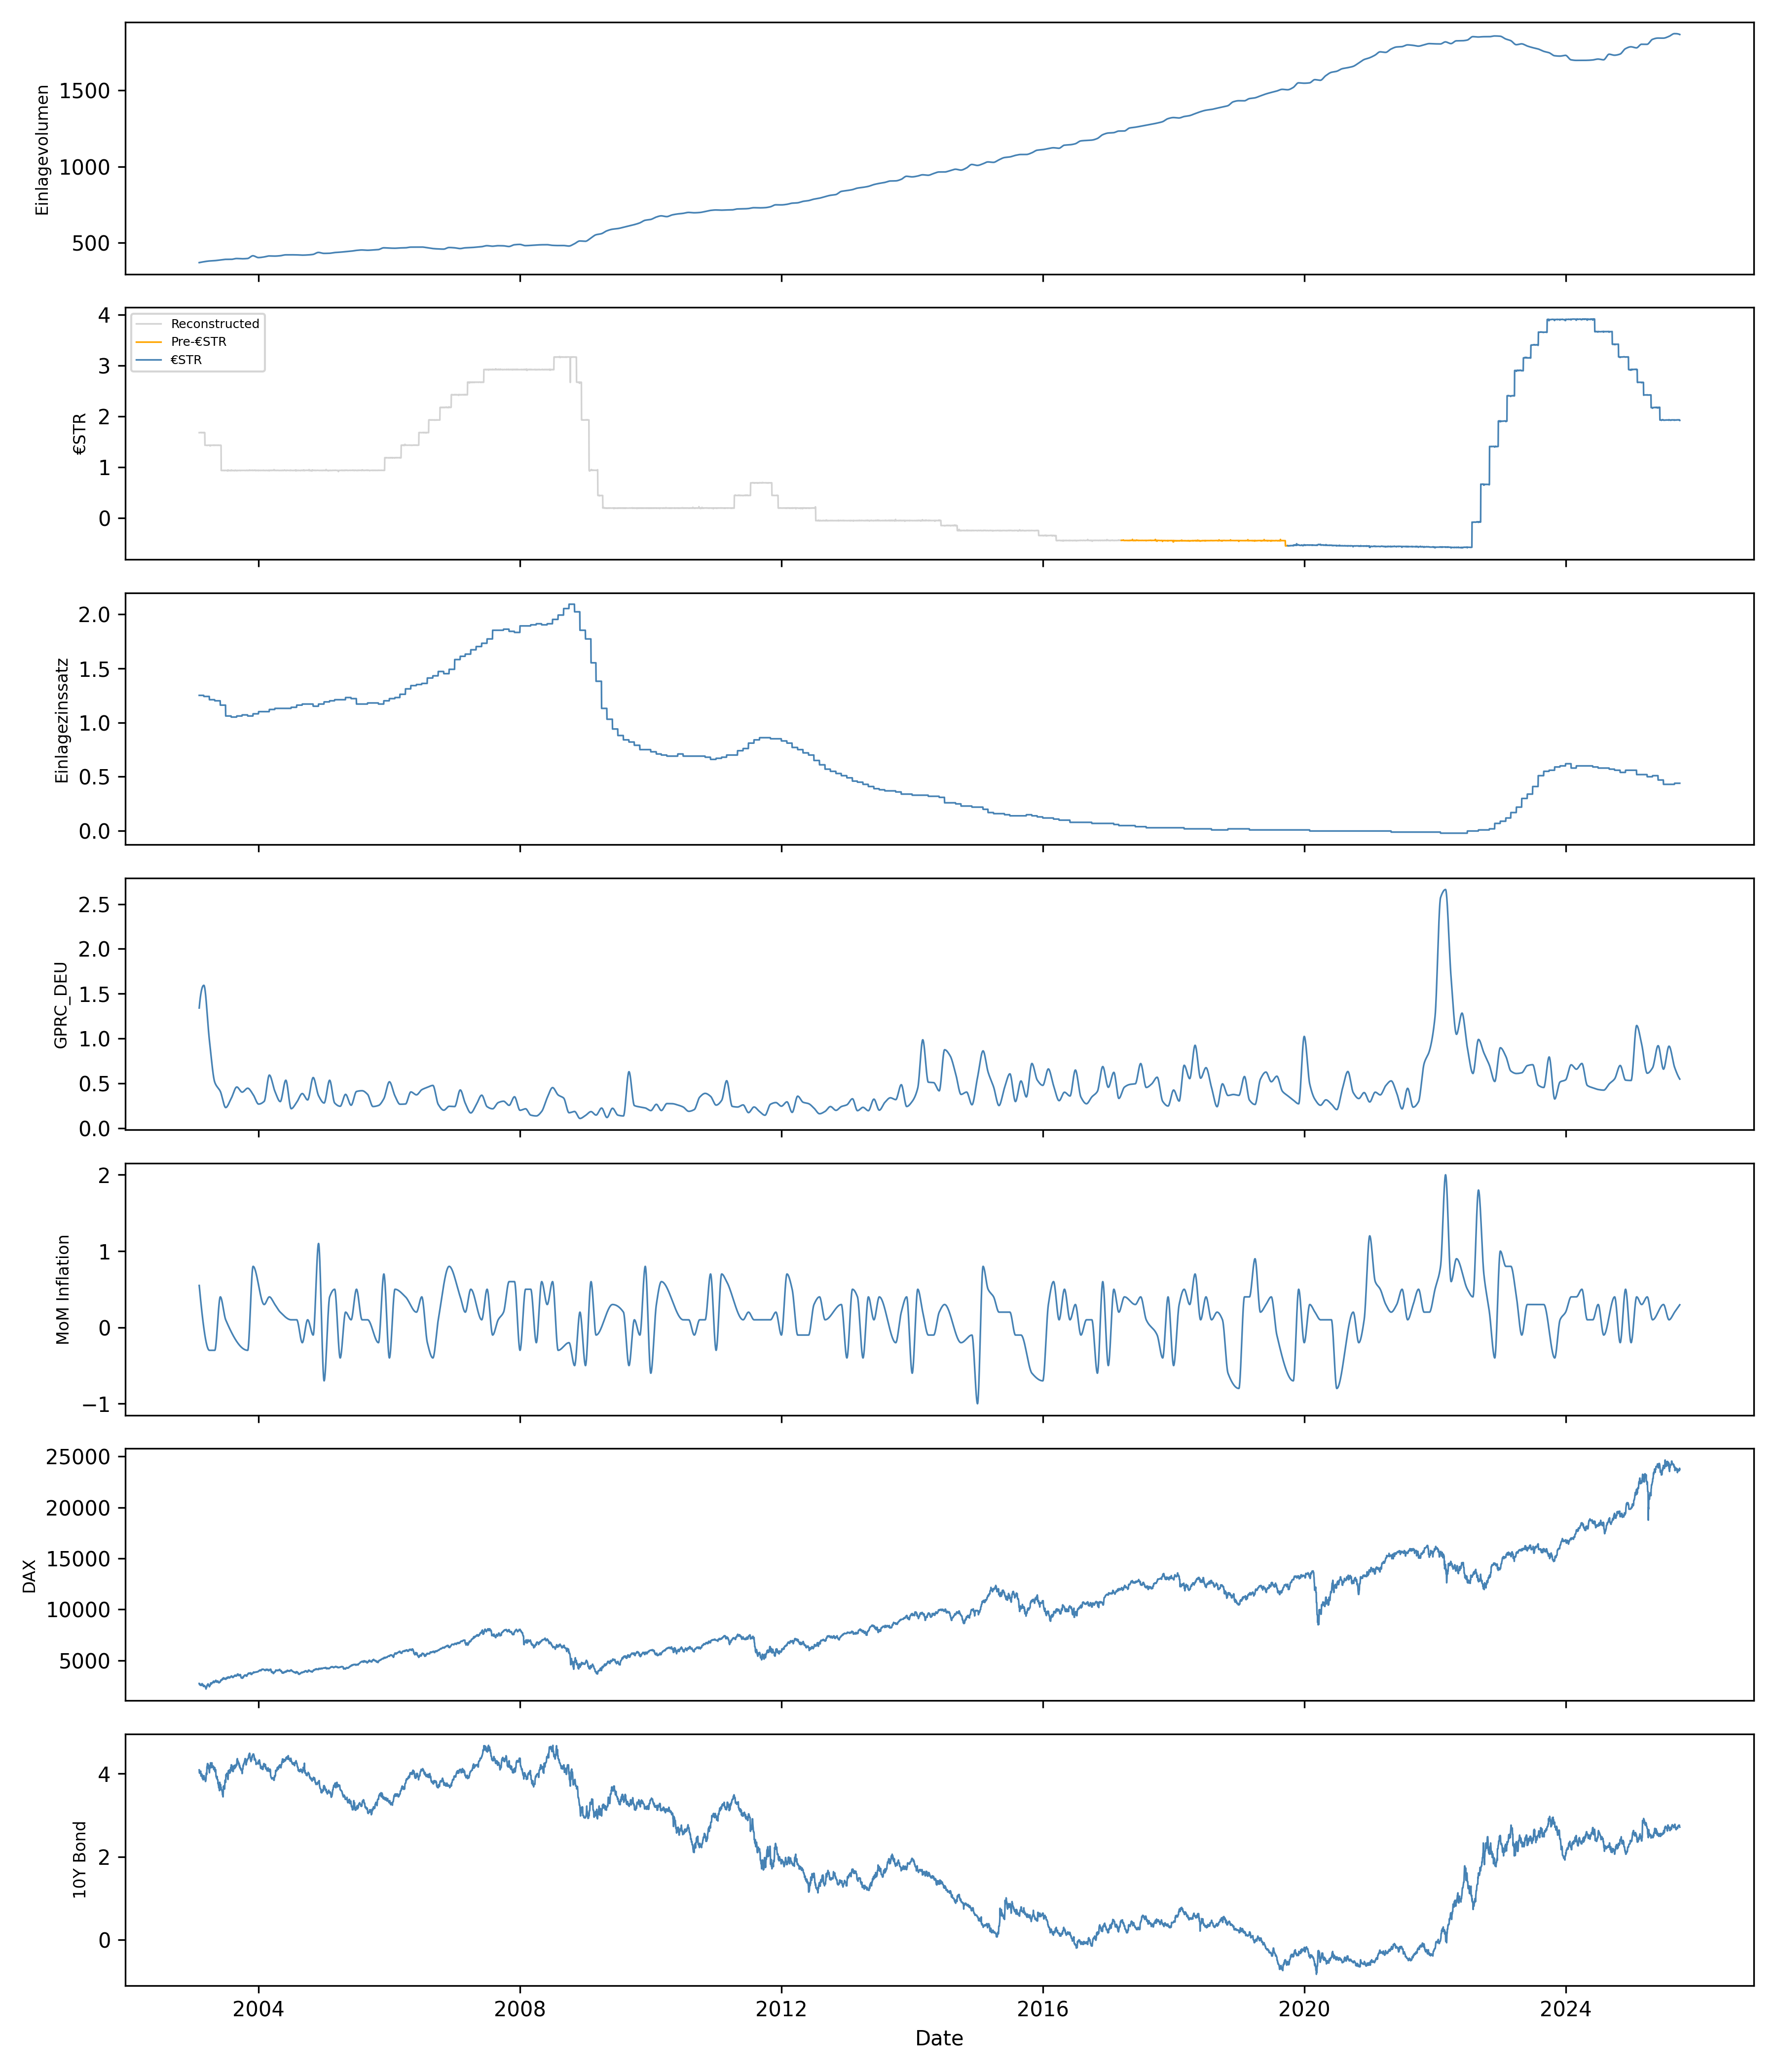
\includegraphics[width=\textwidth]{figures/overview.png}
    \caption{Time series of all variables over the sample period
    January 2003 -- December 2025. All monthly series are shown
    after PCHIP interpolation to daily frequency. The
    $\text{€STR}$ series begins in October 2019 following its
    introduction by the ECB.}
    \label{fig:timeseries_overview}
\end{figure}
% - Jump-problem 
As evident from Figure~\ref{fig:timeseries_overview}, the deposit-volume level exhibits a clear upward trend throughout the timeline, indicating nonstationarity in the mean. To this first differencing is applied, to obtain a stationary target series and to limit accumulating directional errors \citep{box2015},
as illustrated in Figure~\ref{fig:diff_volume}. Second differencing was rejected do to over-differencing.

\begin{figure}[htbp]
    \centering
    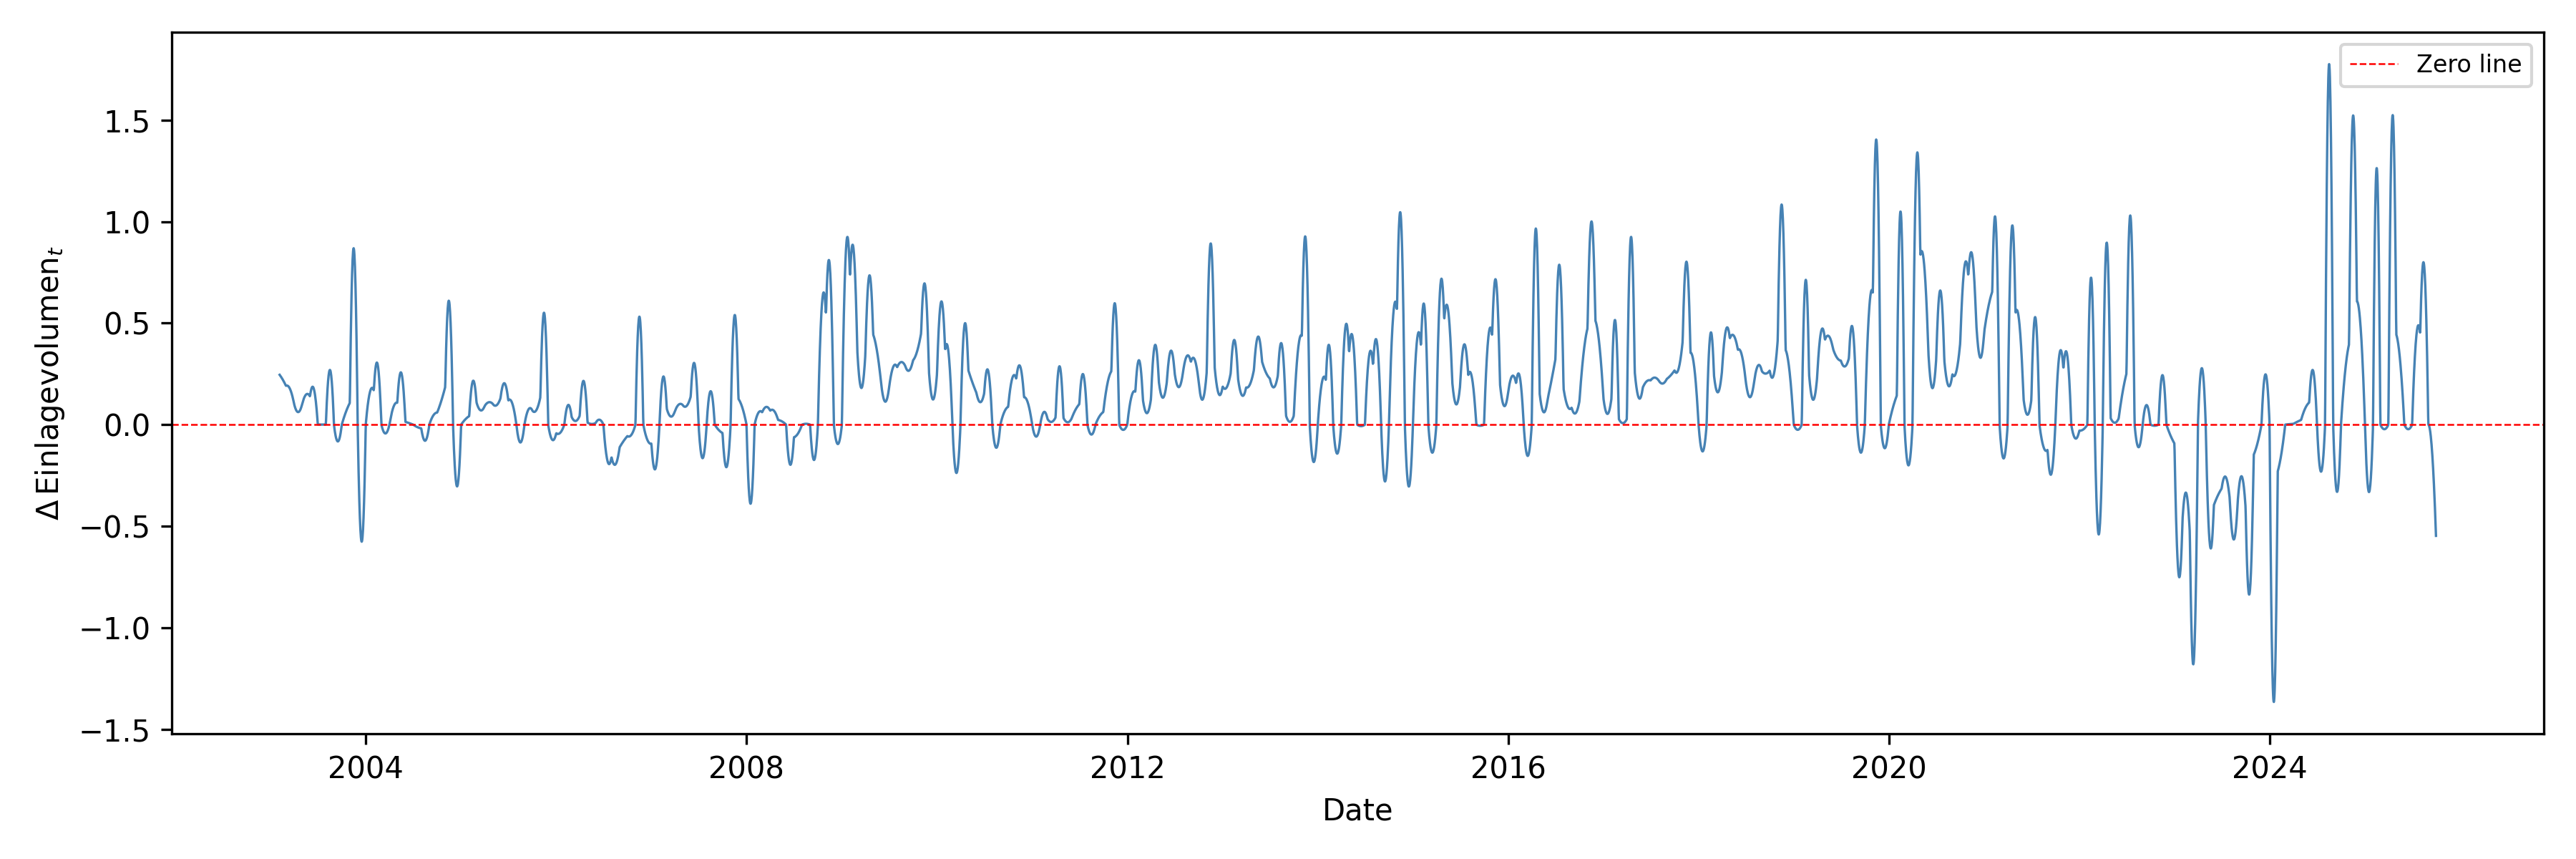
\includegraphics[width=\textwidth]{figures/diff_volume.png}
    \caption{First difference of $\mathrm{Einlagevolumen}_t$ over 
    the full sample period January 2003 -- December 2025. The series 
    fluctuates around zero throughout, confirming stationarity after 
    differencing. Increased volatility from 2022 onward coincides 
    with the ECB interest rate tightening cycle.}
    \label{fig:diff_volume}
\end{figure}
After interpolation to daily frequency, the dataset comprises
$8,276$ observations covering the full sample period January
2003 to September 2025. 

\textit{should we keep it as variables ($STR$ or change to their actual names)}

\section{Forecasting Models}
\subsection{Forecasting Framework}


Let \(y_t\) denote the volume of German household overnight deposits at time
\(t\), and let \(\mathbf{x}_t\) denote the vector of covariates. The objective is to forecast deposit volumes over a
100-day horizon using the information available during the preceding 30 days.

At time of forecast \(t\), the forecasting models use a lookback window of \(L=30\). The information set therefore contains the historical deposit
volume and the selected covariates over the period
\(t-L+1,\ldots,t\). Each model produces the complete vector of predicted
changes for the following \(H=100\) days:
\begin{equation}
    \widehat{\boldsymbol{\Delta y}}_{t+1:t+H}
    =
    f\!\left(
        y_{t-L+1:t},
        \mathbf{x}_{t-L+1:t}
    \right),
    \qquad L=30,\quad H=100.
    \label{eq:forecasting_problem}
\end{equation}

The study therefore applies a direct multi-output forecasting strategy. Each model estimates
all 100 future changes simultaneously rather than recursively one day at a time. The predicted changes are then
converted back into deposit-volume levels according to
\begin{equation*}
    \widehat{y}_{t+h}
    =
    y_t+
    \sum_{j=1}^{h}
    \widehat{\Delta y}_{t+j},
    \qquad h=1,\ldots,H.
    \label{eq:level_reconstruction}
\end{equation*}
\\
\indent Information available up to time $t$ are used
for model estimation and feature scaling. Actual covariate values for those 100 days are not used. For TFT model, while covariates are held constant to the most recent observed value, date-based variables known in advance are provided for the forecast horizon. 

\subsection{Forecasting Models}

\paragraph{Naive benchmarks.}
Random Walk extrapolates the last observed daily change at a constant
rate,
\begin{equation*}
    \hat{y}_{t_0+h} = y_{t_0} + h \cdot \Delta y_{t_0}, \qquad h = 1, \dots, 100,
    \label{eq:naive_rw}
\end{equation*}
which corresponds to an ARIMA$(0,1,0)$ process with drift. Naive Hold instead assumes the level
remains constant, $\hat{y}_{t_0+h} = y_{t_0}$. Both benchmarks are
fully interpretable and require no covariates, serving as a reference against to which compare the more complex models.

\paragraph{Linear Regression (Ridge).}
A multi-output ridge regression maps the flattened 30-day lookback window
to the 100-step forecast vector, regularized by an $\ell_2$
penalty $\alpha$ selected via time-series cross-validation. As a linear model, Ridge provides interpretable results. 

\paragraph{XGBoost.}
Gradient-boosted regression trees are trained on the same flattened
input representation, with hyperparameters (max depth, learning rate,
subsample ratio) \citep{chen2016}. These hyperparameters are selected using chronological time-series cross-validation when tuning is enabled. Boosted trees can capture
non-linear covariate interactions that Ridge cannot
\citep[Ch.~10]{hastie2009}, while remaining moderately interpretable.

\paragraph{Feedforward Neural Network (FFN).}
The untuned FFN with two hidden layers (128, 64 units,
ReLU activation) is trained to directly predict the 100-step output
vector. Training uses Adam optimizer with early stopping based on the last 15\% of
the training window, chronologically. FFN trades interpretability for greater representational flexibility.

\paragraph{Temporal Fusion Transformer (TFT).}
Unlike the sequence models above, the TFT explicitly distinguishes
between \emph{known} future inputs (calendar features: weekday,
month-end indicator, day-of-month) and \emph{unknown} future inputs
(the six macro-financial covariates).
The model is trained with early stopping (patience 5 validation checks) on
validation loss. Despite being the most complex model considered,
the TFT's attention mechanism was explicitly designed by
\citet{lim2021} to offer a degree of interpretability that purely black-box models typically lack.

Each sequence model is fitted \(S\) times with different random seeds to form an
ensemble. When \(S>1\), repeated model fits are combined by averaging their forecasts. Linear regression, FFN, and XGBoost use bootstrap-resampled training
samples and different random seeds, while repeated TFT fits use different
random seeds..

\subsection{Covariate Specifications}
\label{subsec:covariates}

To assess the predictive value of different economic information, each
non-naive model is evaluated using the nine predefined covariate sets shown in
Table~\ref{tab:covariate_sets}. These specifications compare economically
related variable groups, individual interest-rate variables, and parts of
the complete dataset.

\begin{table}[htbp]
    \centering
    \caption{Covariate specifications}
    \label{tab:covariate_sets}
    \begin{tabularx}{\textwidth}{l X}
        \toprule
        Specification & Included variables \\
        \midrule
        All & €STR, deposit rate, geopolitical risk, inflation, DAX,
        and ten-year German government bond yield \\
        Interest rates & €STR and deposit rate \\
        Financial markets & DAX and ten-year government bond yield \\
        Macroeconomic & Geopolitical risk and inflation \\
        Rates and macroeconomy & €STR, deposit rate, geopolitical risk,
        and inflation \\
        Excluding DAX & All variables except DAX \\
        Excluding inflation & All variables except inflation \\
        €STR only & €STR \\
        Deposit rate only & Deposit rate \\
        \bottomrule
    \end{tabularx}
\end{table}


\subsection{Rolling-Origin Evaluation}
\label{subsec:rolling_evaluation}

Forecasting performance is assessed using an expanding-window rolling-origin
design. At each forecast origin \(o_k\), all observations available up to that
date form the training sample, while the following \(H=100\) days form the
evaluation window:
\begin{equation*}
    \mathcal{T}_k=\{1,\ldots,o_k\},
    \qquad
    \mathcal{E}_k=\{o_k+1,\ldots,o_k+H\}.
\end{equation*}
The models are re-estimated at every origin as newly observed data becomes
available. The evaluation uses four origins: 1 January 2009, 1 January 2013,
1 March 2019, and 1 June 2025.

\subsection{Evaluation}
\label{subsec:evaluation_metrics}

Performance is evaluated for both the predicted first differences and the
reconstructed deposit-volume levels. Let \(y_{k,h}\) and
\(\widehat{y}_{k,h}\) denote the observed and predicted volume at horizon \(h\)
after origin \(o_k\). The evaluation metrics are
\begin{align*}
    \operatorname{MAE}_k
    &=
    \frac{1}{H}
    \sum_{h=1}^{H}
    \left|y_{k,h}-\widehat{y}_{k,h}\right|, \\
    \operatorname{RMSE}_k
    &=
    \sqrt{
        \frac{1}{H}
        \sum_{h=1}^{H}
        \left(y_{k,h}-\widehat{y}_{k,h}\right)^2
    }, \\
    R_k^2
    &=
    1-
    \frac{
        \sum_{h=1}^{H}
        \left(y_{k,h}-\widehat{y}_{k,h}\right)^2
    }{
        \sum_{h=1}^{H}
        \left(y_{k,h}-\overline{y}_k\right)^2
    },
\end{align*}
where \(\overline{y}_k\) is the mean observed volume in evaluation window
\(k\). Negative \(R^2\) values indicate performance below the test-window mean
benchmark.

Metrics are calculated separately at each forecast origin and summarized by
their mean and standard deviation across origins. The primary comparison uses
MAE for the reconstructed deposit-volume levels, measured in billions of
euros. RMSE and \(R^2\) provide complementary information, while metrics on
first differences are used as diagnostic measures.




% ---------------------------------------------------------------------------
% 4. Results
% ---------------------------------------------------------------------------
% Guidance (p.25): consider the "rule of three" (roughly: three key
% figures/tables/points is usually enough to make the results section
% land -- avoid overwhelming the reader with every single output).
% Every figure/table must be referenced in the text (e.g. "... in
% Figure 3", "... in Table 2"); state the message of what the reader
% should see, don't just present the plot.
% Guidance on figures (p.28-29):
% - Plots must be printer-friendly (black/white or solid/dashed lines,
%   not color-only encoding).
% - Name axes with units, include a legend.
% - Always state the message of the figure in the surrounding text.
% - Detailed captions: paper is often scanned, so a figure + caption
%   must be understandable WITHOUT reading the surrounding text --
%   name axes/data rows, give setup details (e.g. time range, model).


\section{Results}
\label{sec:results}

\subsection{Forecasting Performance}

Table~\ref{tab:overall_results} reports the best-performing covariate
specification for each model according to mean level MAE. The results are
descriptive because the covariate sets are selected using the same four
evaluation windows on which performance is reported.

\begin{table}[htbp]
\centering
\small
\caption{Forecasting performance across four rolling origins. MAE and RMSE
are measured in EUR billions and reported as mean $\pm$ standard deviation.}
\label{tab:overall_results}
\begin{tabularx}{\textwidth}{l X c c c}
\toprule
Model & Best covariate set & MAE & RMSE & Mean $R^2$ \\
\midrule
Linear model
& All covariates
& $9.36 \pm 11.11$
& $10.26 \pm 12.08$
& $0.178$ \\

TFT
& Macroeconomic
& $10.78 \pm 12.61$
& $12.71 \pm 14.18$
& $-0.361$ \\

Last-change extrapolation
& None
& $11.78 \pm 12.81$
& $14.41 \pm 14.25$
& $-0.564$ \\

FFN
& Macroeconomic
& $11.85 \pm 6.90$
& $15.22 \pm 10.35$
& $-0.605$ \\

XGBoost
& Excluding inflation
& $12.71 \pm 13.28$
& $14.90 \pm 14.79$
& $-0.784$ \\

Constant-level benchmark
& None
& $17.38 \pm 10.13$
& $21.03 \pm 10.52$
& $-2.246$ \\
\bottomrule
\end{tabularx}
\end{table}

The linear model achieved the lowest average MAE and was the only approach
with a positive mean $R^2$. TFT ranked second, followed by the last-change
benchmark. The FFN and XGBoost did not improve upon this simple benchmark on
average, while the constant-level forecast produced the largest errors.
Therefore, greater model complexity did not consistently lead to higher
forecasting accuracy.

\subsection{Effect of Covariate Selection}

The preferred covariate specification differed across models.
The linear model performed best with all six explanatory variables, whereas
the FFN and TFT obtained their lowest MAE using only geopolitical risk and
inflation. XGBoost performed best when inflation was excluded. These findings
suggest that the predictive value of a covariate depends on how the model
represents linear and nonlinear relationships. They should not, however, be
interpreted as evidence of causal effects.

\subsection{Variation Across Forecast Origins}

Forecasting performance varied substantially across the four evaluation
periods, as reflected by the large standard deviations in
Table~\ref{tab:overall_results}. The FFN displayed the lowest variation in
MAE, but its average error remained above those of the linear model and TFT.
The results indicate that no model dominated at every forecast origin and that
model rankings depend on the economic environment.

Because the evaluation contains only four forecast origins, the results should
be interpreted as a comparison across selected historical periods rather than
as evidence of statistical superiority. Nevertheless, the benchmark shows
that simple and interpretable methods remain competitive for forecasting
aggregate household overnight deposits.
\begin{comment}
% ---------------------------------------------------------------------------
% 5. Discussion
% ---------------------------------------------------------------------------
% Guidance (p.25): recommended ideas to cover --
% - Limitations (also feed into Outlook)
% - Managerial implications
% - Future impact
\section{Discussion}
\label{sec:discussion}
% - What does it mean? Interpret the results in context.
% - Why did certain models outperform others?
% - Limitations of the analysis (data, methods, assumptions).
% - Managerial implications for decision-makers.
% - Broader / future impact.
The empirical findings from our rolling-origin benchmark provide crucial insights into how distinct algorithmic architectures handle highly autocorrelated, noisy, and regime-shifting financial time series over a $100$-day forecasting horizon. While modern data science literature frequently advocates for deep non-linear models, our evaluation across four distinct macroeconomic interest rate regimes ($2009$--$2025$) reveals a more complex reality. 

This section critically evaluates the performance, structural strengths, and architectural constraints of all six benchmarked models: Feedforward Neural Networks (FFN), Regularized Linear Regression (LinReg), Temporal Fusion Transformers (TFT), Gradient Boosted Trees (XGBoost), Naive Random Walk (Naive RW), and Naive Hold.

\subsection{Feedforward Neural Networks (FFN): High Capacity and Feature Sensitivity}
The Feedforward Neural Network achieved the lowest overall Mean Absolute Error ($\text{MAE} = 7.25$~Bn.~\texteuro), representing a $38\%$ reduction in prediction error relative to the Naive RW baseline. The model's hidden architecture ($128 \times 64$ fully connected nodes) successfully captured complex, non-linear relationships between broad macroeconomic indicators and deposit flows—such as non-linear behavioral shifts during negative rate regimes.

However, cross-regime variance analysis reveals that the FFN is highly sensitive to the chosen feature space. When supplied with rich, multi-dimensional macroeconomic inputs (\texttt{nur\_makro}), the network generalized exceptionally well. Conversely, when restricted to single-rate covariates (e.g., \texttt{nur\_zinsen}), performance degraded rapidly, producing large error spikes. This highlights that deep architectures require multi-vector regularizing inputs to prevent hidden layers from memorizing historical baseline trends that fail to persist across future rolling origins.

\subsection{Regularized Linear Regression (LinReg): The Gold Standard for Stability}
While ranking second in absolute MAE ($8.41$~Bn.~\texteuro), the Linear Regression model fitted with Ridge ($L_2$) regularization demonstrated the highest out-of-sample coefficient of determination ($R^2 = 0.255$) among all evaluated approaches. 

The structural advantage of $L_2$-regularized linear models in cumulative horizon forecasting lies in their smooth penalty mechanism. When predicting daily volume differences ($\Delta y_t$) over $H = 100$ steps, small daily estimation errors compound linearly or quadratically during final volume reconstruction:
\begin{equation}
    \hat{y}_{t_0+h} = y_{t_0} + \sum_{k=1}^{h} \Delta \hat{y}_{t_0+k}
\end{equation}
The Ridge penalty shrinks non-essential feature weights toward zero, effectively filtering out high-frequency noise. Consequently, during extreme regime shifts—such as the transition from near-zero rates in 2013 to aggressive tightening in 2025—LinReg maintained low error variance ($\pm 11.61$~Bn.~\texteuro), outperforming all complex models in cross-regime stability.

\subsection{Temporal Fusion Transformer (TFT): Architectural Overhead vs. Input Constraints}
The Temporal Fusion Transformer ranked third overall ($\text{MAE} = 9.33$~Bn.~\texteuro, $R^2 = -0.006$). Although TFT is designed specifically for multi-horizon time series forecasting via attention mechanisms and variable selection networks, its full potential was constrained by the strict ex-post evaluation setup.

To prevent look-ahead bias, future values of dynamic covariates were held constant using a naive-hold assumption over the $100$-day horizon. As a result, TFT’s temporal self-attention layers received static input sequences for future steps, neutralizing its primary structural mechanism for dynamic pattern recognition. While TFT successfully outperformed tree-based models and naive baselines, its heavy parameterization added computational overhead without delivering superior accuracy over simpler FFN or Ridge models under static future covariate assumptions.

\subsection{Gradient Boosted Trees (XGBoost): The Extrapolation Trap}
XGBoost exhibited severe structural limitations in this experiment, yielding a negative out-of-sample $R^2$ ($-0.307$) and a higher average MAE ($10.56$~Bn.~\texteuro). 

The primary cause of XGBoost's underperformance is the inherent inability of decision trees to extrapolate continuous trends beyond the bounded feature space of the training data. Tree-based algorithms partition the feature space into orthogonal hyper-rectangles, predicting a constant step-value within each leaf node. When forecasting during historical volume highs (such as the $2025$ rate surge), XGBoost cannot project a continuing upward slope; it caps predictions at the maximum values observed in the training set. Furthermore, because XGBoost was trained via direct multi-output regression ($100$ separate tree ensembles), distant forecast steps ($h \to 100$) accumulated significant variance during summation.

\subsection{Naive Baselines: Essential Anchors for Model Validation}
The inclusion of non-parametric naive benchmarks provides crucial context for evaluating model value:
\begin{itemize}
    \item \textbf{Naive Random Walk (Naive RW):} Assumes zero daily change ($\Delta y = 0$), resulting in an average MAE of $11.78$~Bn.~\texteuro{} ($R^2 = -0.564$). While competitive during tranquil market conditions, it fails completely during macroeconomic pivots. All primary ML models (FFN, LinReg, TFT, XGBoost) statistically outperformed Naive RW, confirming that ML models extract genuine economic signals.
    \item \textbf{Naive Hold:} Projects the historical average change, resulting in the worst overall performance ($\text{MAE} = 17.38$~Bn.~\texteuro, $R^2 = -2.246$). This confirms that static trend projection is entirely unsuited for multi-step banking deposit horizons.
\end{itemize}

%\begin{figure}[htbp]
    %\centering
    %\includegraphics[width=0.85\textwidth]%{figures/error_accumulation_horizon.png}
    %\caption{Cumulative forecast error accumulation across all six evaluated model architectures over the $100$-day forecasting horizon.}
%    \label{fig:error_accumulation}
%\end{figure}

\subsection{Managerial Implications and Practical Takeaways}
Table~\ref{tab:model_discussion_summary} summarizes the empirical rankings and architectural trade-offs across all six evaluated models for bank asset-liability management (ALM).

\begin{table}[htbp]
\centering
\caption{Comprehensive Benchmark Summary across 4 Interest Rate Regimes ($2009$--$2025$).}
\label{tab:model_discussion_summary}
\begin{tabular}{c l l c c c}
\toprule
\textbf{Rank} & \textbf{Model} & \textbf{Best Covariate Set} & \textbf{Mean MAE [Bn. \texteuro]} & \textbf{Mean $R^2$} & \textbf{vs. Naive RW} \\
\midrule
\#1 & \textbf{FFN} & \texttt{nur\_makro} & \textbf{7.25} $\pm$ 8.84 & 0.181 & $-38\%$ \\
\#2 & \textbf{LinReg (Ridge)} & \texttt{alle} & 8.41 $\pm$ 11.61 & \textbf{0.255} & $-29\%$ \\
\#3 & \textbf{TFT} & \texttt{nur\_makro} & 9.33 $\pm$ 12.87 & $-0.006$ & $-21\%$ \\
\#4 & \textbf{XGBoost} & \texttt{nur\_einlagezins} & 10.56 $\pm$ 11.37 & $-0.307$ & $-10\%$ \\
\#5 & \textbf{Naive RW} & \texttt{naive} & 11.78 $\pm$ 12.81 & $-0.564$ & Baseline \\
\#6 & \textbf{Naive Hold} & \texttt{naive} & 17.38 $\pm$ 10.13 & $-2.246$ & $+48\%$ worse \\
\bottomrule
\end{tabular}
\end{table}

For practical bank liquidity management, \textbf{Regularized Linear Regression} offers the most reliable tradeoff between strong interpretability, rapid execution, and high regime-shift stability ($R^2 = 0.255$). Meanwhile, the \textbf{Feedforward Neural Network} provides superior absolute precision when comprehensive macroeconomic indicators are available to guide its non-linear layers.
\end{comment}


% ---------------------------------------------------------------------------
% 6. Conclusion and Outlook
% ---------------------------------------------------------------------------
% Guidance (p.26), three-part structure:
%   1. Repeat problem and its relevance
%   2. Repeat contribution, incl. quantitative results
%   3. [Optional] Outlook on further research steps
\section{Conclusion and Outlook}
\label{sec:conclusion}

% --- Part 1: Problem + relevance, briefly restated ---

% --- Part 2: Contribution + key quantitative results ---

% --- Part 3: Outlook / future work ---

% ---------------------------------------------------------------------------
% Acknowledgements (journals only -- optional for this course deliverable)
% ---------------------------------------------------------------------------
% \section*{Acknowledgements}

% ---------------------------------------------------------------------------
% Bibliography
% ---------------------------------------------------------------------------
% Prefer "good" references (course guidance, p.9): peer-reviewed
% journals/conferences, English, from the same or a closely related
% domain, ideally from ranked outlets (e.g. VHB JOURQUAL, FT50,
% Handelsblatt ranking). Use books mainly for background, and web
% sources mainly as data sources -- not as the primary evidence base.
%
% Option A: natbib + a .bib file (recommended; use a reference manager
% such as Citavi, Zotero, or EndNote to build references.bib)
\bibliographystyle{apalike}
\bibliography{references}

% Option B: manual thebibliography (quick start, replace with natbib
% once you have enough sources -- course guideline: ~10-40 references
% cited, scanning up to ~100)
%\bibliographystyle{apalike}
%\bibliography{references}

% ---------------------------------------------------------------------------
% Appendices
% ---------------------------------------------------------------------------
\appendix
\section{Appendix: Additional Figures and Tables}
\label{app:additional}
% Any supplementary material that doesn't fit in the main text.

\section{Appendix: Code}
\label{app:code}
% Code can be attached and counts towards the length requirement
% (22,000-33,300 characters per the seminar description).
\begin{lstlisting}[language=Python, caption={Example: model fitting excerpt}]
def fit_sequence_model(model_name, X_train, y_train, seed=SEED):
    # ...
    pass
\end{lstlisting}

\end{document}
